\section{Functionality description}
This section goes over the app functionalities and how they are designed and implemented.

\subsection{Login}
This is a section going over logging in to the application. If it is the first time the user uses the application they will have to create an account with username
and password. Otherwise only password is required. If user inserts password that does not match their corresponding password stored in database the 
"Invalid password" message is displayed. If the password is correct, the main window of the application is shown.

This is implemented in the file \texttt{main.py} in the function \texttt{start\_app()}.

\subsection{File selection}
Selecting files is handled by the button \texttt{Choose a file to be sent}. When the button is pressed, a dialog window is opened where the user can select
a file. The implementation of this is done using module \texttt{filedialog} from \texttt{tkinter} library. If a file is not selected, the window wont let them
select only path that is not pointing to a file. If the window is closed without selecting the filepath is kept empty.

The code itself can be seen in file \texttt{file\_share/app/app.py} in the function \texttt{get\_file()}.

\subsection{Listing users}
There are two functionalities that are related to listing users. The first one is listing all non-friend users that are in the database. The second one 
is listing all users that user has added as a friends. Both of these open a new windows where the users are listed. The difference between these two windows
is that in window where non-friend users are listed, there is a button to add them as a friend.

The list friends functionality is simpler and it is done by retrieving all users from the database and filtering out the ones that are friends with the user.
The method that handles this is the \texttt{get\_all\_users} from \texttt{file\_share/database/\_\_init.py\_\_}, where there is friend parameter which is by default set to \texttt{True}.\\
The non-friends is a bit more complicated first the list of all users except friends is collected from the database. It is listed in the window. If user wants 
to add a friend, he selects that user from the list and pressed button "Befriend this user", this calls a function \texttt{befriend} in \texttt{file\_share/database/\_\_init.py\_\_}.
This adds the user as a friend by setting the \texttt{is\_friend} attribute to \texttt{True}.

\subsection{File sending initialization}
For this core functionality there is attached a flow chart for easier understandability. It is implemented in function \texttt{send\_file} in \texttt{file\_share/app/app.py}.
The function first checks if the file for transfer is selected, if that is so then the file is prepared for transfer and file transfer is attepmted sending is done by 
function \texttt{send\_or\_store\_file} from \texttt{file\_share/sender/sender.py}. As a return there is a \texttt{SendStatus} object, which is enum created for this application,
there are 5 states that the object can be in, those can be viewed in \texttt{file\_share/definitions/enums.py}. Based on the the state of the user which is passed to the function,
the file will either be sent, stored in outgoing queue or nothing will happen.\\

If the file is to be stored then it is scheduled to be added to files table in the database using \texttt{store\_file} from \texttt{file\_share/database/\_\_init.py\_\_}.

\begin{figure}[ht]
    \centering
    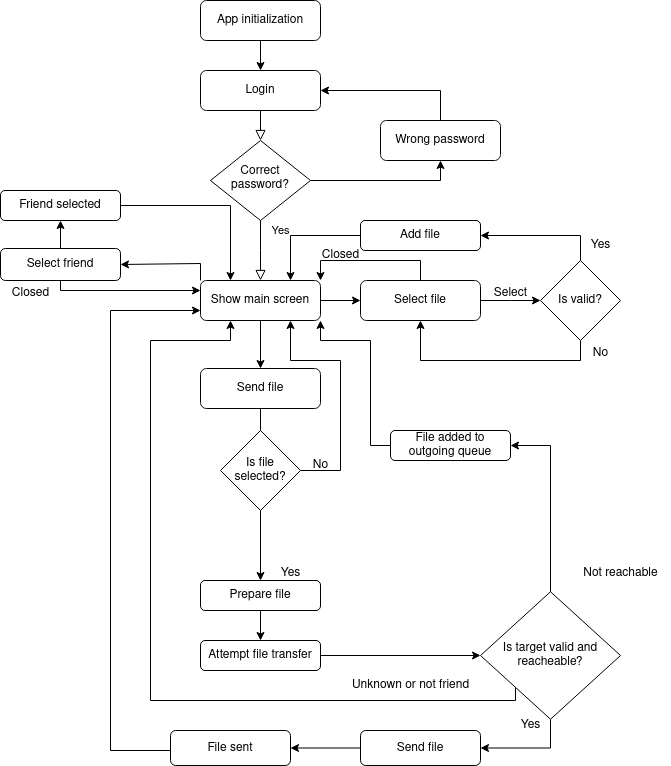
\includegraphics[scale = 0.5]{images/filesending.png}
    \caption{Flowchart of file sending initialization}
    \label{fig:flowchart}
\end{figure}
\subsection{File sending}
In this section the process of file transfer itself is described. It is accompanied by a figure that shows the sides of the communication and the steps
that each of the sides takes.\\
This whole process is based on using a one time use API key which is generated by the recieving side of the communication. This key is then used by the sender in 
the header of the file transfer as a verification of the communication. 
Firstly the sender extracts from the file object that is passed as a parameter the username of target user, then on the basis of this username retrieves the
address of this user from database, unless the file has address override in it. In which case the override adress is used as a target address.\\
Then the SSL context of given username is taken and using aiohttp session a request is made to the target user. The target then verifies if the sender is a friend,
if not then exception 401 is raised and the communication is terminated by this exception. If the sender is a known friend, then an API key is generated, encoded using the senders public 
key extracted from their certificate and sent back to the sender as a response. This verification and key generating is done in \texttt{file\_share/receiver/receiver\_api.py} in method \texttt{auth()}.\\
When sender recieves this API key, it is decrypted using the senders private key, then a FormData object is created, the file is added to it and finally a sending
is done with this FormData object, where as the header is included this API key.\\
On the recieving side, when the file transfer is done the API key is removed from database as it is one time use only. If the key is not found in database then
a 401 exception is raised and this ends the communication. Otherwise a new file object is created with the incoming attribute set to True, the object is timestamped,
and sender username is associated with it. Then it is added to the database table and the file's name is returned as a response.\\

\begin{figure}
    \centering
    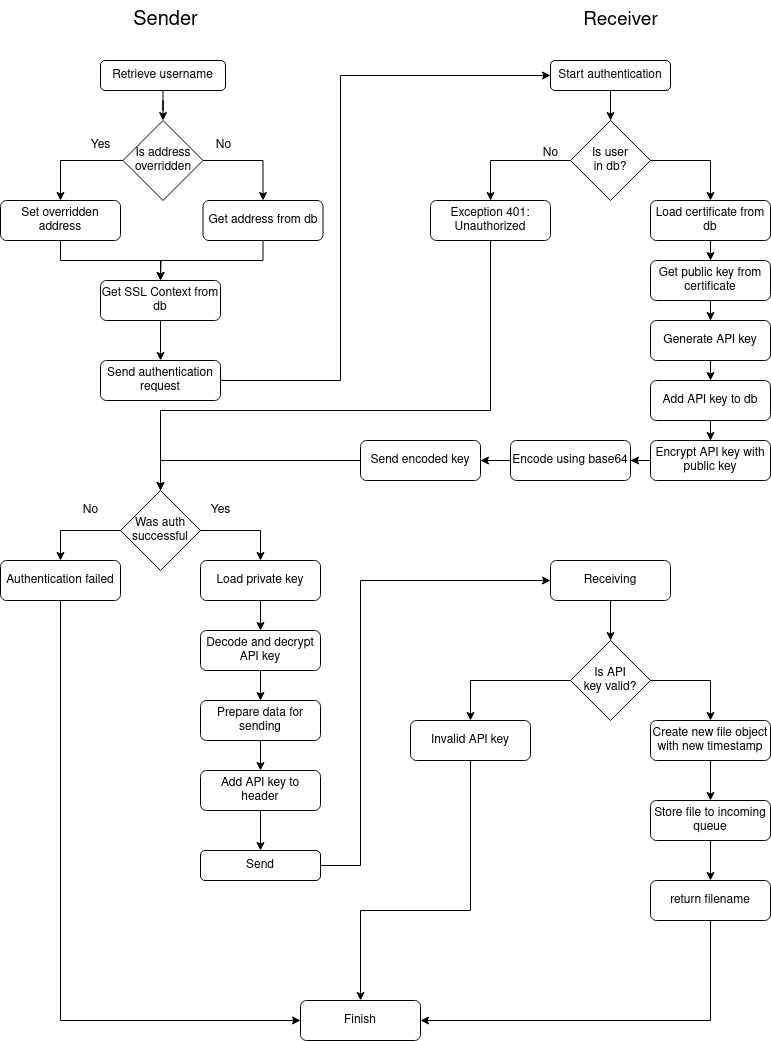
\includegraphics[scale = 0.5]{images/file_send.png}
    \caption{Flowchart of file transfer}
    \label{fig:filetransfer}
\end{figure}